\documentclass{pnastwo}


\usepackage{graphicx}
\usepackage{amsmath}



\begin{document}
	
\title{Supplemental Information: The relationship between dN/dS and scaled selection coefficients}
	
	\author{Stephanie J. Spielman\affil{1}{Department of Integrative Biology, Center for Computational Biology and Bioinformatics, and Institute of Cellular and Molecular Biology.
			The University of Texas at Austin, Austin, TX 78712, USA.}
		\and
		Claus O. Wilke\affil{1}{}}

\maketitle

\bigskip
\bigskip
\bigskip
\bigskip

\centerline{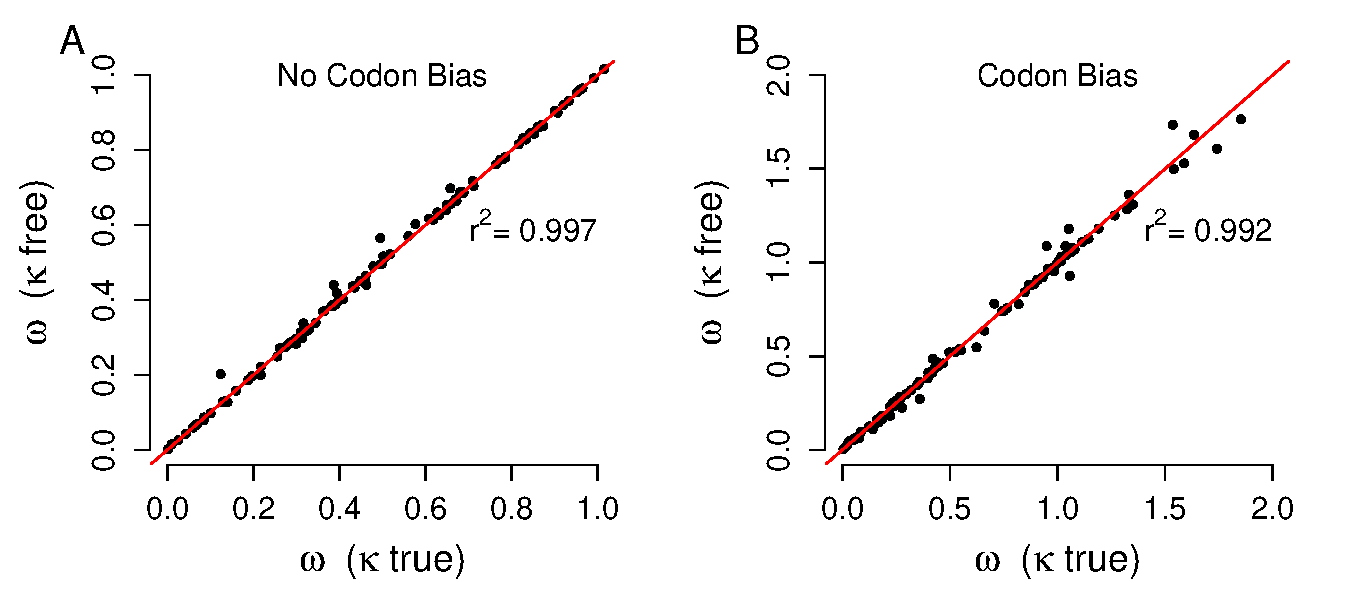
\includegraphics[width=5.5in]{figures/SI/omega_kappafree_kappatrue.pdf}}
\noindent Figure S1. Caption!
	
\bigskip
\bigskip
\bigskip
\bigskip


\centerline{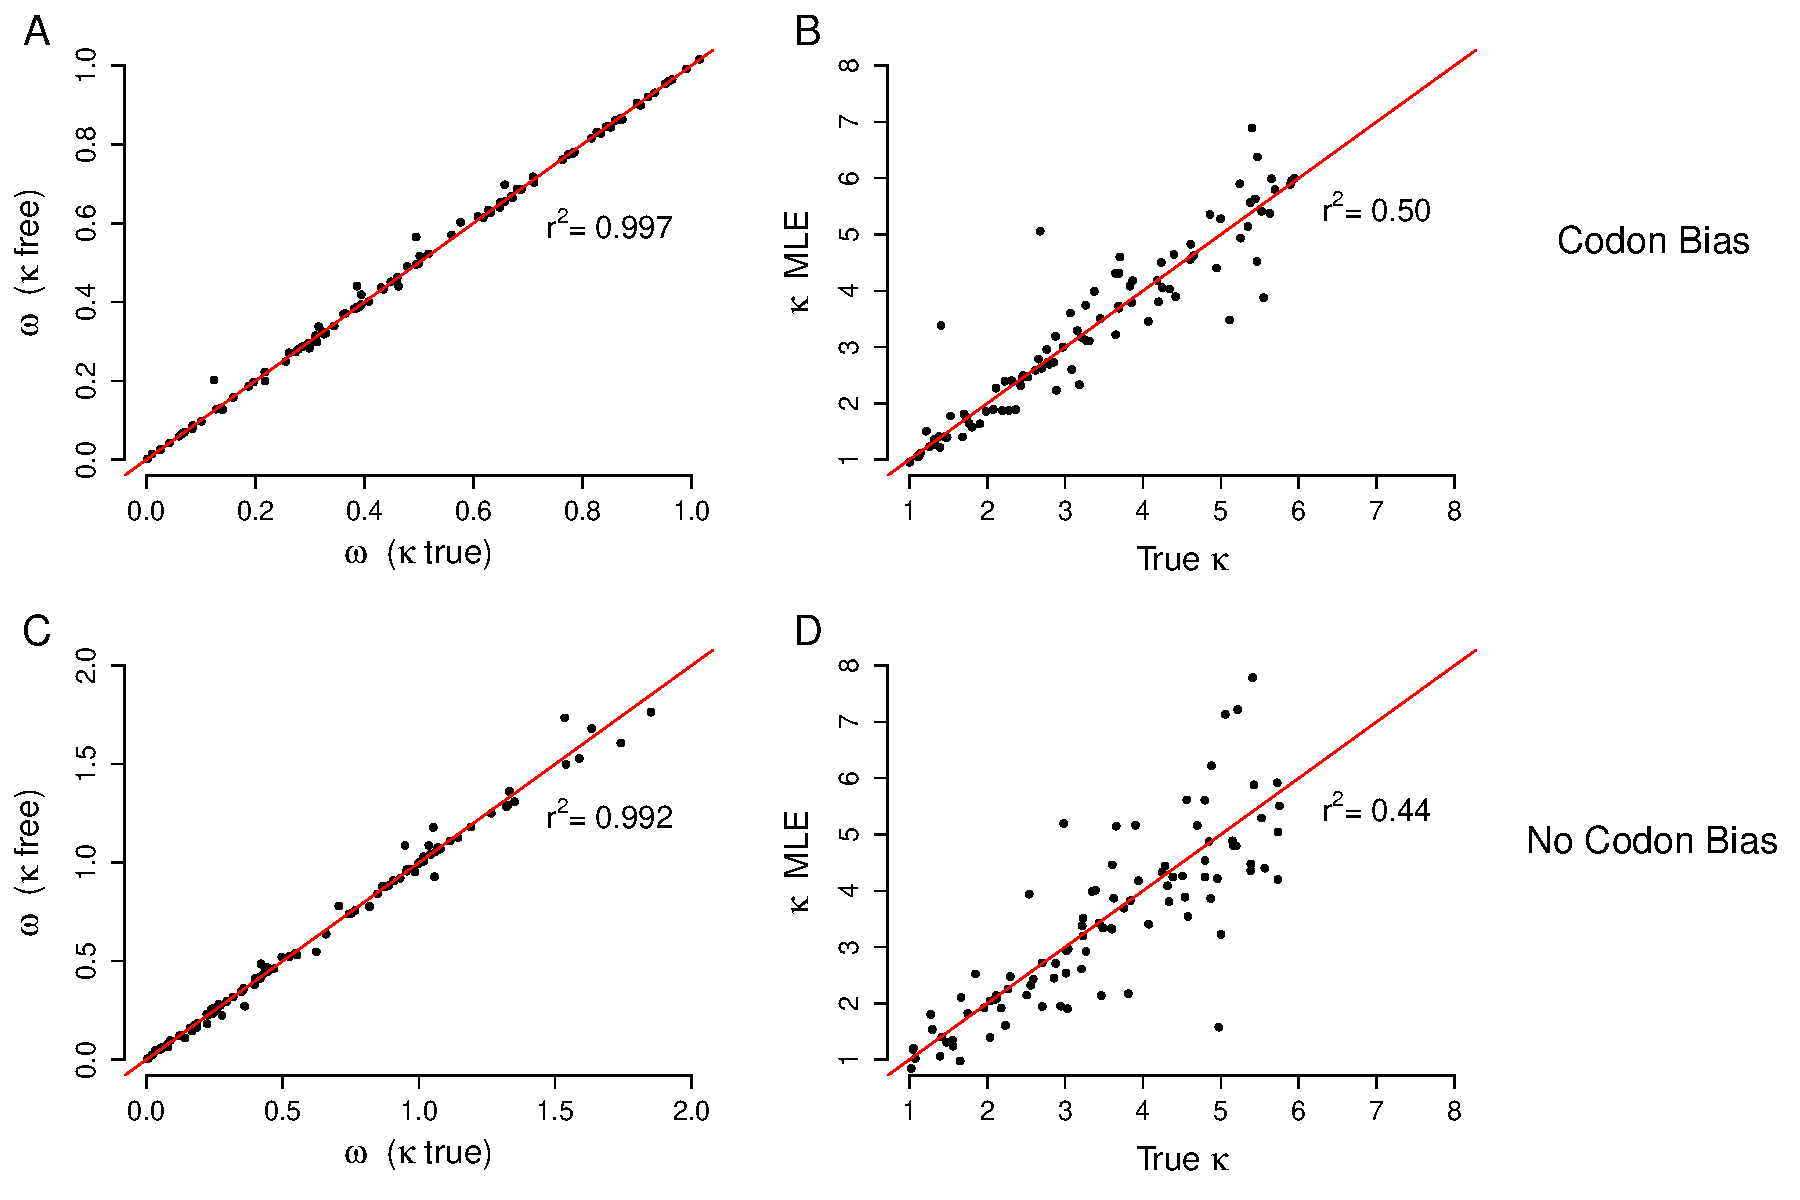
\includegraphics[width=5.5in]{figures/SI/kappa_regressions.pdf}}
\noindent Figure S2. Caption!

\clearpage
\newpage

\vspace*{-1.5cm}{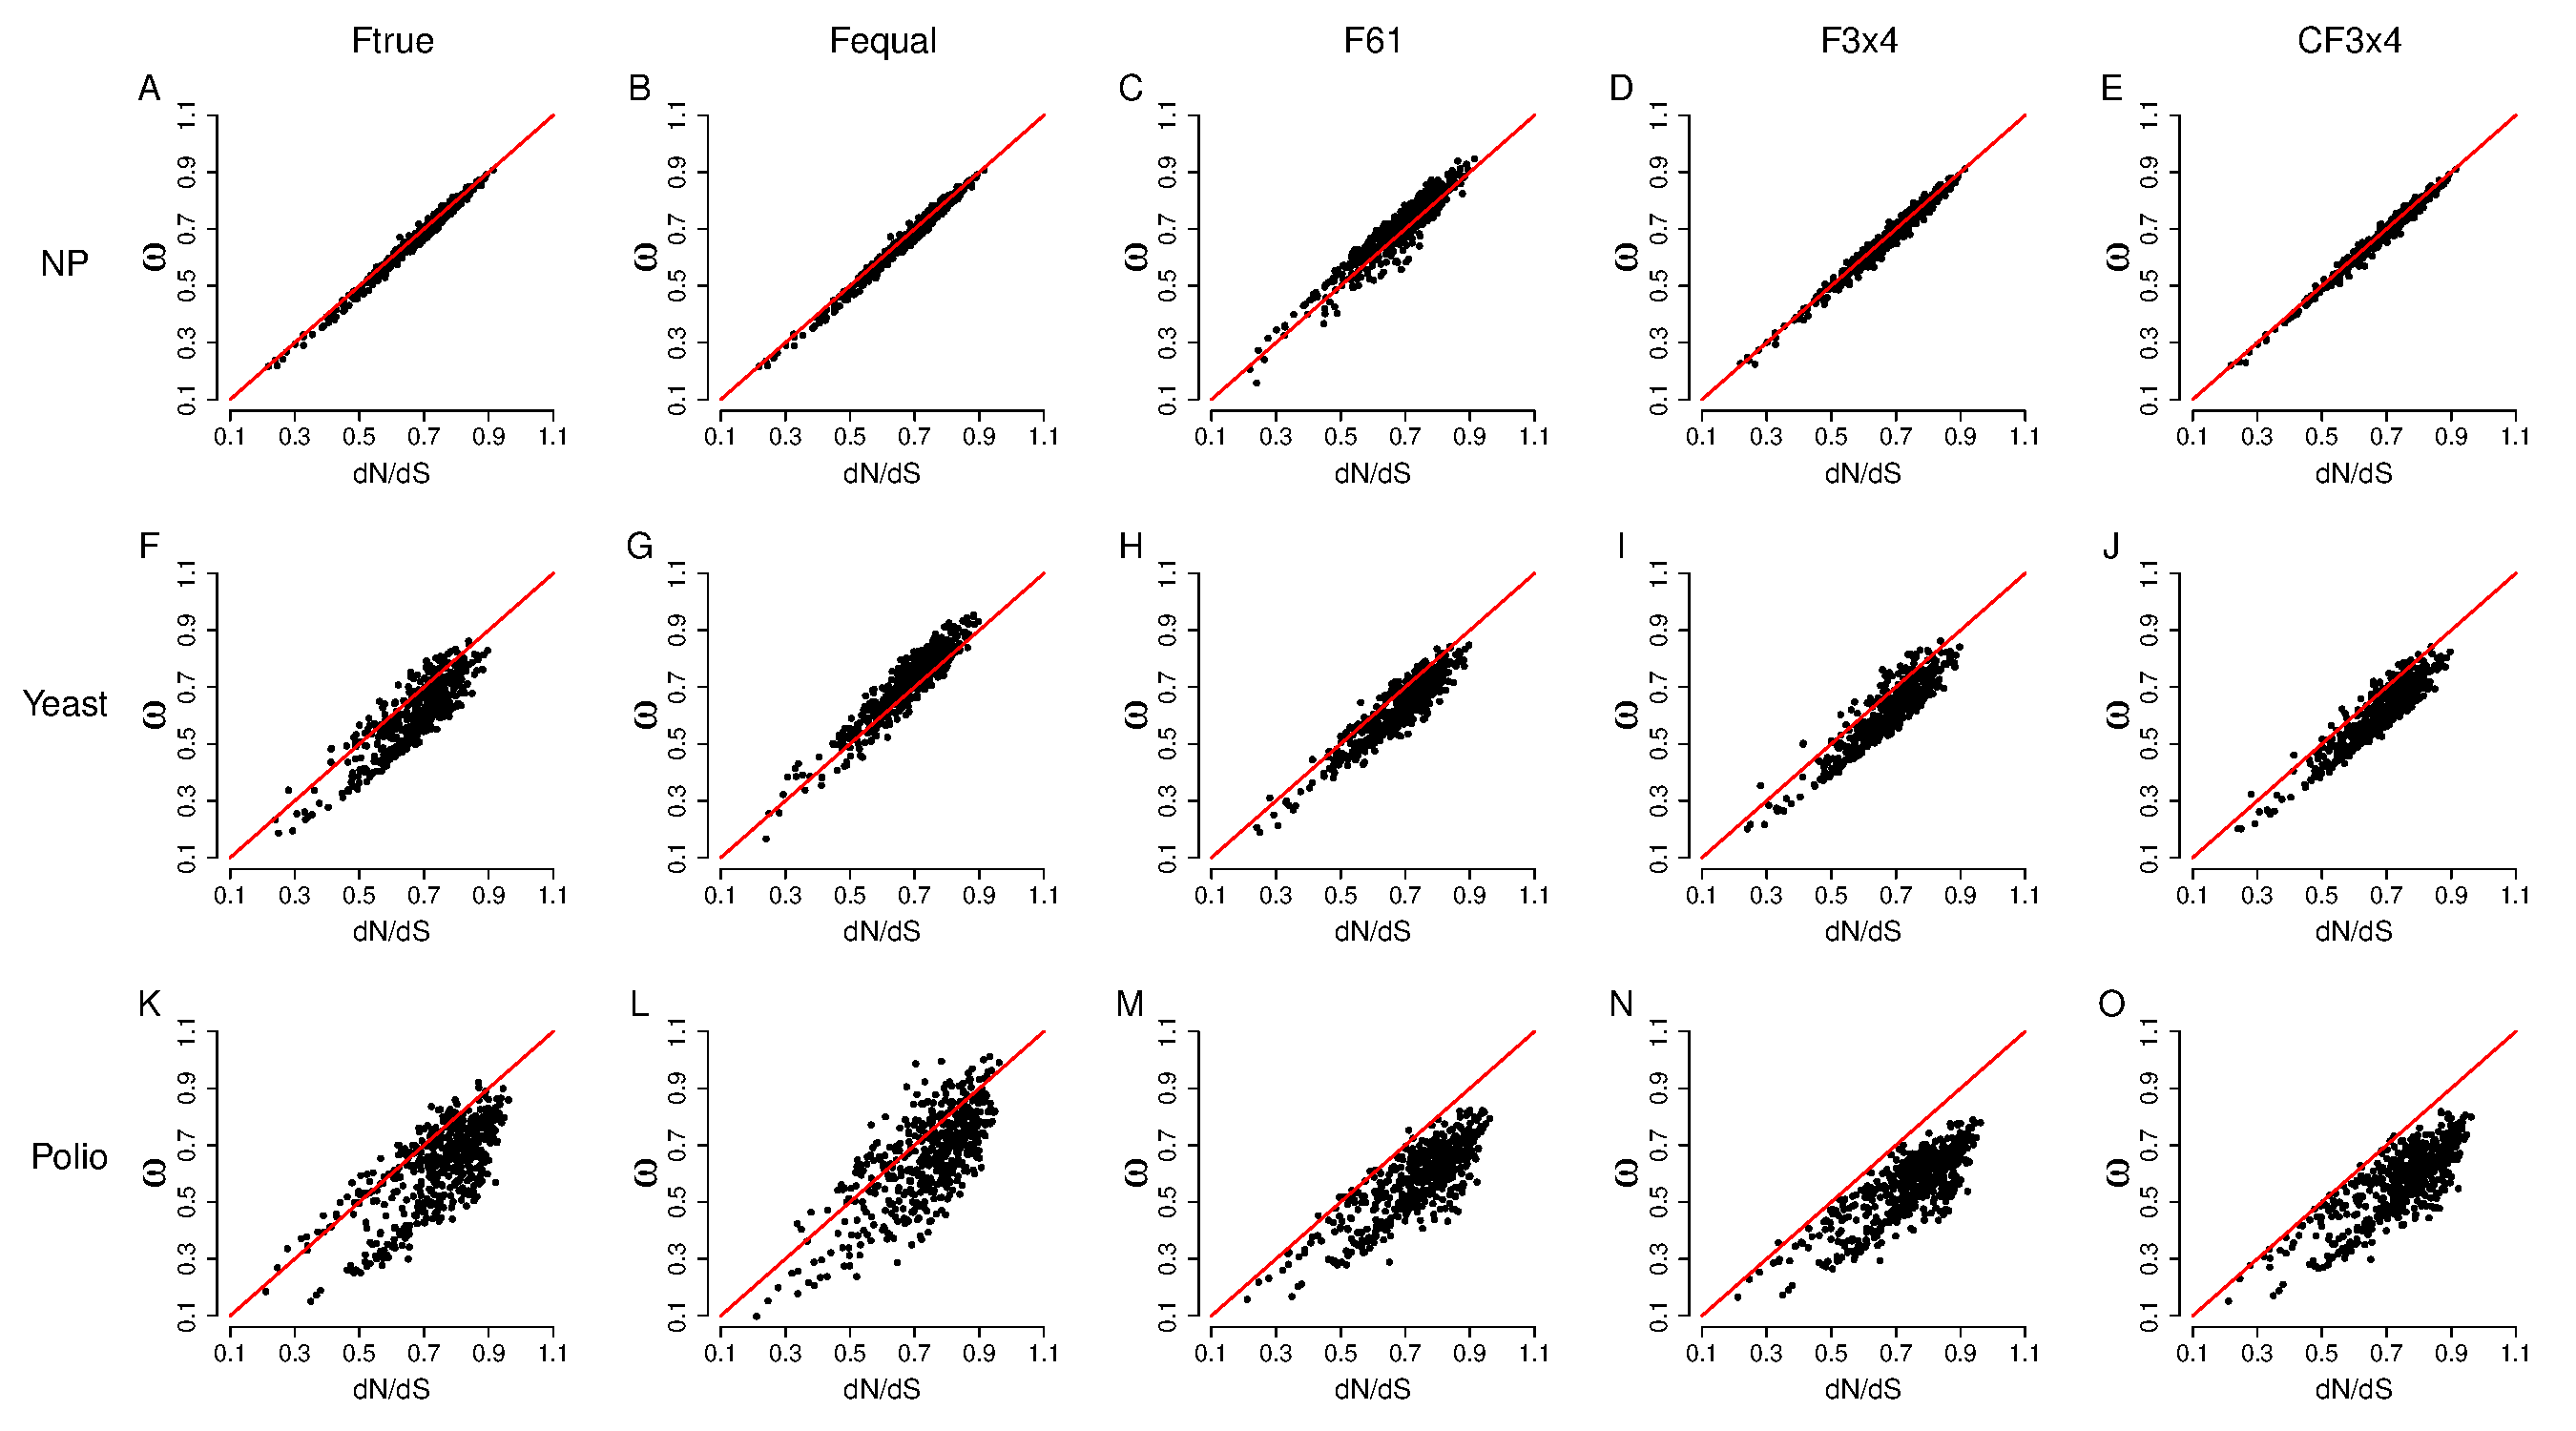
\includegraphics[width=9.5in, angle=90]{figures/SI/nyp_fspecs_full.pdf}
\noindent Figure S3. Caption!

\clearpage
\newpage

\noindent Table S1. NYP BIAS. 
\begin{table}[htbp]
	\begin{tabular}{c c c c c c}
		\hline\noalign{\smallskip}
		& \multicolumn{5}{c}{M0 model codon frequency parameterization} \\
		\cline{2-6}\noalign{\medskip}
		Mutation rate & Ftrue & Fequal & F61 & F3x4 & CF3x4 \\
		\hline\noalign{\smallskip}
		NP & -0.0097 & -0.011 & 0.02 & -0.0063 & -0.0084 \\
		Yeast & -0.072 & 0.029 & -0.056 & -0.66 & -0.73 \\
		Polio & -0.12 & -0.082 & -0.16 & -0.18 & -0.17 \\
		\noalign{\smallskip}\hline\noalign{\smallskip}
	\end{tabular}
\end{table}	

\bigskip
\bigskip
\bigskip
\bigskip
\bigskip

\noindent Table S2. NYP $r^2$. 
\begin{table}[htbp]
	\begin{tabular}{c c c c c c}
		\hline\noalign{\smallskip}
		& \multicolumn{5}{c}{M0 model codon frequency parameterization} \\
		\cline{2-6}\noalign{\medskip}
		Mutation rate & Ftrue & Fequal & F61 & F3x4 & CF3x4 \\
		\hline\noalign{\smallskip}
		NP & 0.988 & 0.986 & 0.902 & 0.975 & 0.986 \\
		Yeast & 0.740 & 0.877 & 0.850 & 0.820 & 0.848 \\
		Polio & 0.537 & 0.519 & 0.659 & 0.671 & 0.641 \\
		\noalign{\smallskip}\hline\noalign{\smallskip}
	\end{tabular}
\end{table}	



\end{document}
